\subsection{Threshold optimization}

The choice of the optimal cutoff for binarization is based on the $F_1$ score computed on full-size images. In practice, the DL models are evaluated on a grid of values and the best one is selected according to the \textit{Kneedle} method \cite{kneedle}. 
The same is done for the non-ML approach, with the only difference of considering the cutoff yielding the maximum $F_1$ value. 
The resultant thresholds is then used to assess performances on the test set.
\begin{figure}[h]
\centerline{
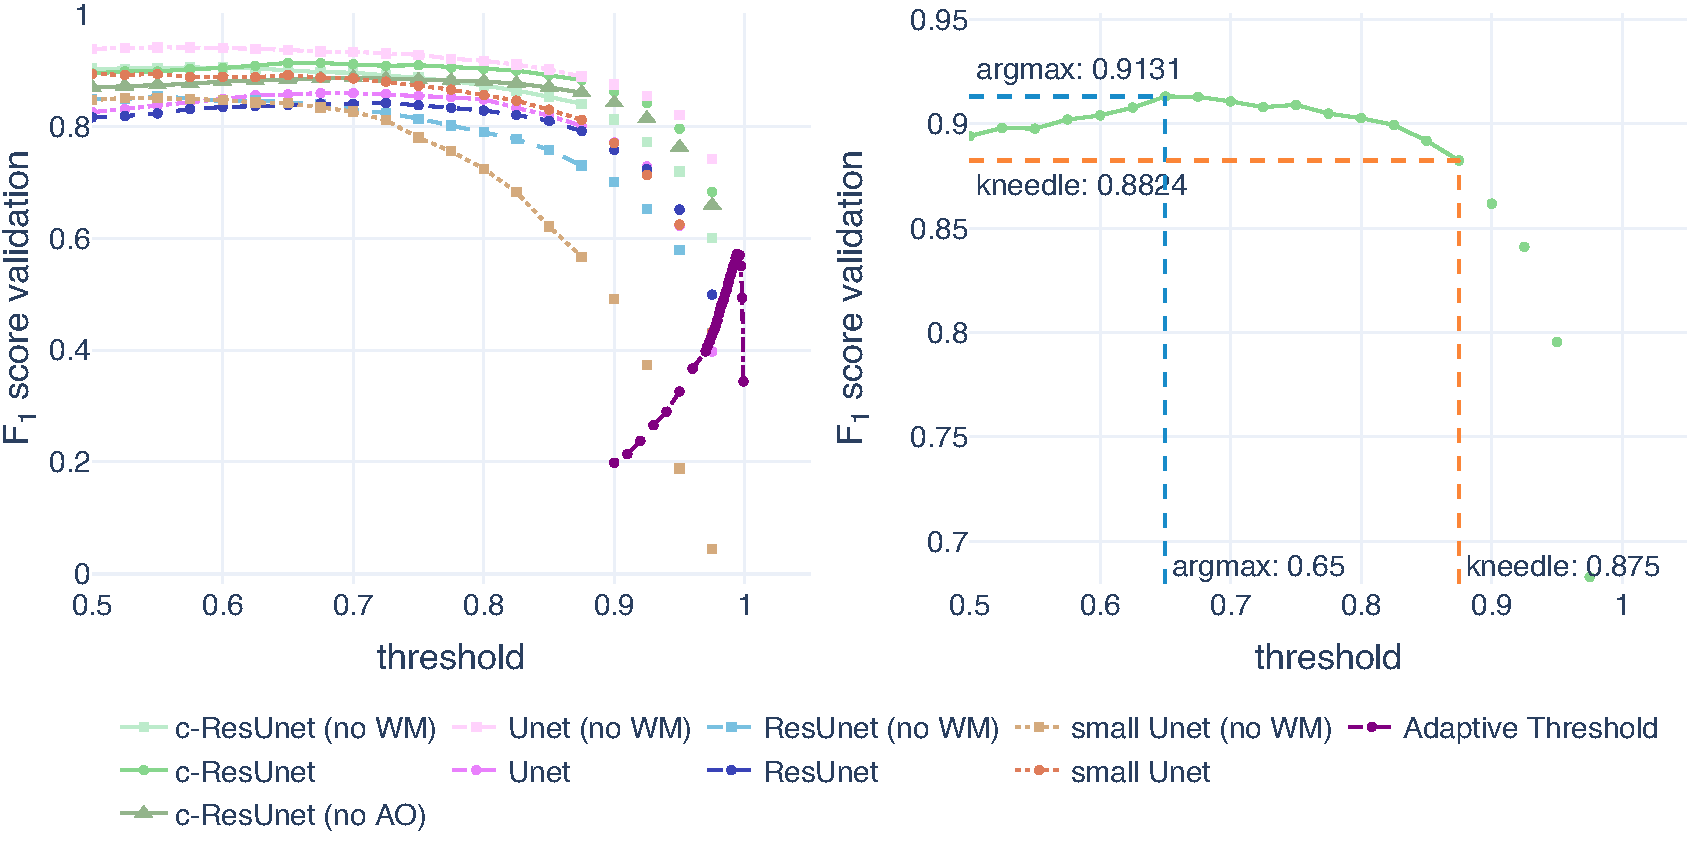
\includegraphics[width=\textwidth]{figures/130_methods/F1_optimization.pdf}
}
\caption{\textbf{Threshold optimization.} On the left, the $F_{1}$ score computed on validation images as a function of the cutoff for thresholding.
On the right, the same is reported for the c-ResUnet to illustrate the selection of the best threshold for binarization according to \textit{argmax} (blue) and \textit{kneedle} (red) methods
% in the case of  the c-ResUnet model
} 
\label{fig:thresh_opt}
\end{figure}
Although the ultimate goal is retrieving the counts, we rely on detection performance to enforce accurate recognition and avoid spurious balancing between false positives and false negatives -- which are indistinguishable from the counts.
Also, full-size images (as opposed to crops) are used to simulate better the model performance in a real-world scenario.
% If the distance between their centroids was less than a fixed threshold (50 pixels, i.e. average cell diameter), the predicted element was considered a true positive; a false negative otherwise.
% Detected items not associated with any target were considered as false positives instead.

\Cref{fig:thresh_opt} shows the optimization results. On the left, we can see how each model performance varies in the validation set as a function of the cutoff for binarization.
For the adaptive thresholding approach, only very high thresholds lead to acceptable performances and we observe a sharp peak followed by a rapid decrease thereafter.
% Even though lower thresholds work best for all DL models, the $F_1$ curves are rather flat after their peaks. 
On the contrary, all DL models work best for lower thresholds and present $F_1$ curves which are rather flat after their peaks.
Thus, increasing the cutoff allows focusing only on predictions whereby the model is very confident, with just a slight loss in overall performance.
Also, good practices in natural science applications suggest being conservative with counts and only consider clearly stained cells.
For these reasons, we opted for the \textit{argmax} value (0.994) for the baseline approach, while we resorted to the \textit{Kneedle} method \cite{kneedle} for the selection of the optimal DL threshold. 
An example of that choice in the case of c-ResUnet is reported in \cref{fig:thresh_opt} (right).